\label{sec:algorithm-imageorientationindicator}

W obrazie \DICOM jest pośrednio zapisana informacja o ułożeniu obrazu względem pacjenta.
Celem algorytmu jest określenie jaką pozycje przyjmuje pacjent w stosunku do sceny, tak aby można było wyświetlić ta pozycje na scenie.

\subsubsection{Format zapisu informacji o orientacji obrazu}

\par
Informacje o orientacji oraz pozycji względem pacjenta znajdują się w odpowiednio w tagach \dicomtag{ImageOrientation}{0020}{0037} i \dicomtag{ImagePosition}{0020}{0032}.

\par
Standard \DICOM zdefiniował ułożenie osi we współrzędnych kartezjańskich następująco:
\begin{itemize}
    \item \quotett{x} --- oś przechodząca od prawej do lewej strony pacjenta, \dataword{L} oznacza zwrot zgodny z osią, a \dataword{R} oznacza zwrot przeciwny

    \item \quotett{y} --- oś przechodząca od przodu do tyłu pacjenta, \dataword{P} oznacza zwrot zgodny z osią, a \dataword{A} oznacza zwrot przeciwny

    \item \quotett{z} --- oś przechodząca od dołu do góry pacjenta, \dataword{H} oznacza zwrot zgodny z osią, a \dataword{F} oznacza zwrot przeciwny

\end{itemize}

\begin{figure}[!htbp]
    \centering
    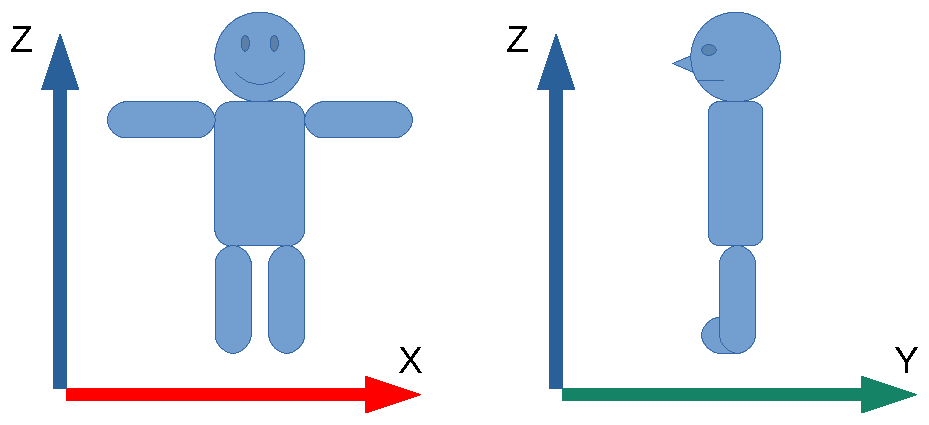
\includegraphics[width=0.7\textwidth]{img/imageorientationindicator-003.pdf}
    \caption{Wizualizacja układu osi współrzędnych kartezjańskich pacjenta. Zdjęcie własne.}
    \label{fig:imageorientationindicator2}
\end{figure}

\par
Wartość \dicomtag{ImageOrientation}{0020}{0037} składa się z sześciu liczb, opowiednio oznaczanych dalej X\textsubscript{x}, X\textsubscript{y}, X\textsubscript{z}, Y\textsubscript{x}, Y\textsubscript{y}, Y\textsubscript{z}.
Standard DICOM definiuje, że te dane mają być z interpretowane w następujący sposób:
\[
    \begin{bmatrix}
        P_x \\ P_y \\ P_z \\ 1
    \end{bmatrix}
    =
    \begin{bmatrix}
        X_x\Delta_i & Y_x\Delta_j & 0 & S_x \\
        X_y\Delta_i & Y_y\Delta_j & 0 & S_y \\
        X_z\Delta_i & Y_z\Delta_j & 0 & S_z \\
        0           & 0           & 0 & 1
    \end{bmatrix}
    \begin{bmatrix}
        i \\ j \\ 0 \\ 1
    \end{bmatrix}
    =
    M
    \begin{bmatrix}
        i \\ j \\ 0 \\ 1
    \end{bmatrix}
\]
gdzie:
\begin{itemize}
    \item $P_{xyz}$ --- koordynaty woksela (i,j) w współrzędnych obrazu wyrażone w milimetrach
    \item $S_{xyz}$ --- trzy wartości z elementu ze znacznikiem \dicomtag{ImagePosition}{0020}{0032}. Oznacza punkt pozycji pacjenta wyrażony w milimetrach w stosunku do urządzenia wykonującego pomiar.
    \item $X_{xyz}$ --- trzy pierwsze wartości z \dicomtag{ImageOrientation}{0020}{0037}
    \item $Y_{xyz}$ --- trzy ostatnie wartości z \dicomtag{ImageOrientation}{0020}{0037}
    \item $i$ i $j$ --- oznaczają współrzędne na macierzy obrazu, odpowiednio kolumnę i wiersz. Zero oznacza początek.
    \item $\Delta_i$ i $\Delta_j$ --- rzeczywista wielkość piksela obrazu wyrażoną w milimetrach, w algorytmie wyznaczania strony pacjenta ta wartość, może wynosić 1, ponieważ odpowiada za skale
\end{itemize}

Praktycznie rzecz biorąc, pierwsza macierz to wektor reprezentujący pozycję pacjenta.
Druga jest to transformata.
Trzecia to pozycja na obrazie.

\subsubsection{Wyznaczanie pozycji pacjenta}

Interesuje nas wyznaczenie pozycji sześciu (punktów) na płaszczyźnie obrazu.
Załóżmy, że pacjent znajduje się w środku układu współżędnych i jest nieskończenie mały.
Możemy więc zdefiniować sześć punktów o następujących współrzędnych, dalej używanych pod nazwą $PatientPosition$, które będą odpowiadały stroną pacjenta:
\begin{itemize}
    \item \quotett{R} - $[-1, 0, 0, 1]$
    \item \quotett{L} - $[+1, 0, 0, 1]$
    \item \quotett{A} - $[0, -1, 0, 1]$
    \item \quotett{P} - $[0, +1, 0, 1]$
    \item \quotett{F} - $[0, 0, -1, 1]$
    \item \quotett{H} - $[0, 0, +1, 1]$
\end{itemize}
Punkty $PatientPosition$ odpowiadają punktom $P_{xyz}$ z równania ze standardu \DICOM.

\par
UWAGA: Wszystkie obliczenia odbywają się w współrzędnych jednorodnych.

\par
Na równaniu z poprzedniego punktu wykonuje takie przekształcenie:
\[PatientPosition = imgMatrix * ScenePosition\]
\[imgMatrix^{-1} * PatientPosition = imgMatrix^{-1} * imgMatrix * ScenePosition\]
\[imgMatrix^{-1} * PatientPosition = ScenePosition\]
\[ScenePosition = imgMatrix^{-1} * PatientPosition\]
gdzie:
\begin{itemize}
    \item $imgMatrix$ --- macierz przekształcenia obrazu, o której będzie dalej
    \item $ScenePosition$ --- pozycja na obrazie, która naz interesuje
    \item $PatientPosition$ --- któryś z punktów względem pacjenta.
\end{itemize}
\par
Wygląd macierzy $imgMatrix$:
\[
    \begin{bmatrix}
        X_x & Y_x & 0 & 0 \\
        X_y & Y_y & 0 & 0 \\
        X_z & Y_z & 0 & 0 \\
        0   & 0   & 0 & 1
    \end{bmatrix}
\]
Powyższa macierz różni się od macierzy definiowanej w standardzie.
Po pierwsze PikselSpacing został pominięty, a konkretniej nadałem mu wartość 1.
Po drugie pozycja z \dicomtag{ImagePosition}{0020}{0032} została zrównana do punktu zerowego, dzięki temu, wynik też będzie względem punktu zero.
Wyznaczenie macierzy $imgMatrix$ jest jednorazowe.

\par
Po wyznaczeniu sześciu punktów $ScenePosition$, po jednej dla każdego punktu względem pacjenta są zapisywane. $ScenePosition$ odpowiada pozycji punktów na obrazie w pozycji startowej.

\par
Na scenie, której jest wyświetlany obraz, użytkownik, może obracać obraz o dowolny kąt, według własnego uznania.
Te przekształcenia, są realizowane za pomocą macierzy rotacji, dalej znana jako $rotateTransform$.
Macierz $rotateTransform$ jest przesyłana do naszego obiektu \sokarclass{ImageOrientationIndicator} za każdym razem kiedy zostanie zmieniona.

\par
Ostateczne wyznaczenie pozycji punktów pacjent na obrazie odbywa sie przez przemnożenie lewostronne $rotateTransform$ i $ScenePosition$.
\[rotateTransform * ScenePosition\]
Wyznaczane jest w ten sposób pozycja sześciu punktów pacjenta na płaszczyźnie sceny wyświetlanej.
Następnie określane jest na, której z ośmiu części płaszczyzny jest umieszczony dany punkt, podział płaszczyzny jest widoczny na rysunku \ref{fig:imageorientationindicator4}.
Tej płaszczyźnie nadawany jest tytuł w postaci litery, która oznacza stronę pacjenta.
Jeżeli punkt znajduje się w centrum, na przecięciu osi, to oznacza, że punkt znajduje się za lub przed ekranem, więc jest pomijany.
Następnie do czterech pól wyświetlających zostają wstawione następujące teksty:
\begin{itemize}
    \item lewe pole: tytuł części 7, tytuł części 0 i tytuł części 1
    \item górne pole: tytuł części 1, tytuł części 2 i tytuł części 3
    \item prawe pole: tytuł części 3, tytuł części 4 i tytuł części 5
    \item dolne pole: tytuł części 7, tytuł części 6 i tytuł części 5
\end{itemize}

\par
Przykład:\\
Punkt \quotett{H}, czyli punkt reprezentujący kierunek głowy, został przypisany do części 1 i odpowiednio \quotett{L} do części 7, \quotett{R} do części 3 i \quotett{F} do części 5.
Punkty \quotett{A} i \quotett{P} zostały pominięte ponieważ znalazły się na środku.
Do lewego pola wstawiany jest tekst \quotett{HL}, do górnego \quotett{HR}, do prawego \quotett{RF} i do dolnego \quotett{LF}.

\begin{figure}[!htbp]
    \centering
    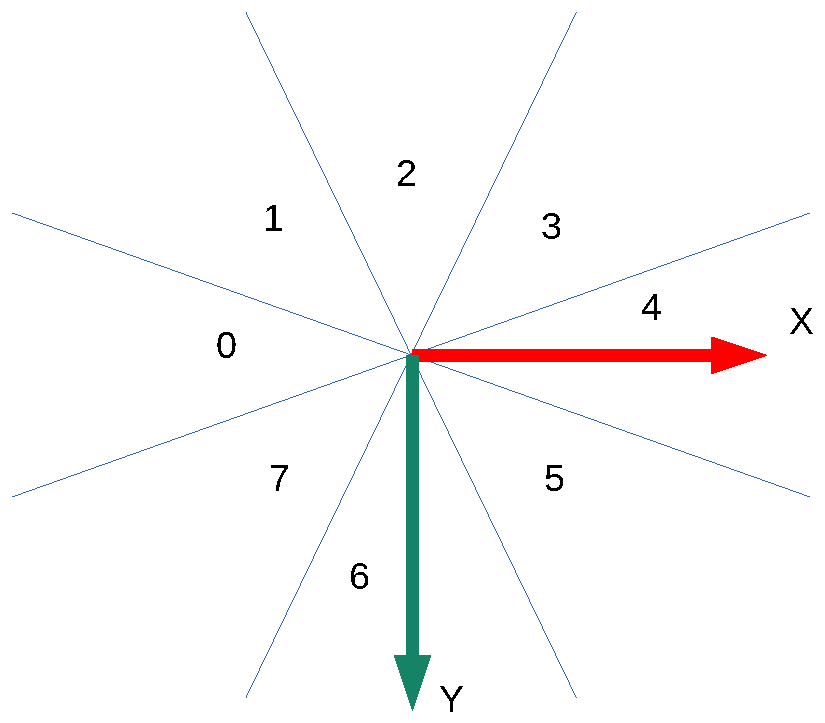
\includegraphics[width=0.5\textwidth]{img/imageorientationindicator-004.pdf}
    \caption{Podział płaszczyzny sceny. Wyróżniono osiem części. Zdjęcie własne.} 
    \label{fig:imageorientationindicator4}
\end{figure}

\par
Przykład można zobaczyć na rysunku \ref{fig:imageorientationindicator1}.
Na obrazie widzimy, że lewa strona pacjenta znajduje się po prawej stronie obrazu, prawa strona pacjenta po lewej, góra pacjenta na górnej części obrazu.
Wynika z tego, że obraz przedstawia pacjenta skierowanego twarzą do nas.

\begin{figure}[!htbp]
    \centering
    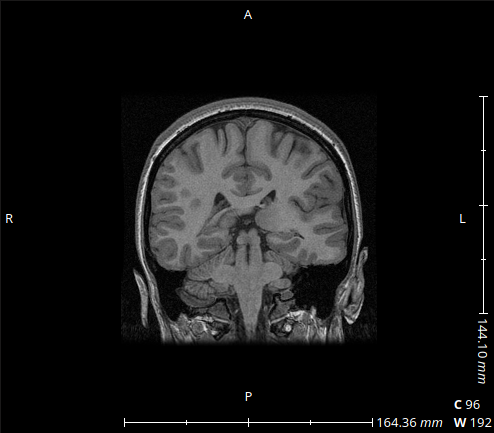
\includegraphics[width=100mm]{img/imageorientationindicator-002.png}
    \caption{Przykładowy obraz medyczny (przekrój głowy MR) z oznaczeniem orientacji obrazu z apomocą liter A, P, R, L, F, H. Zdjęcie własne.}
    \label{fig:imageorientationindicator1}
\end{figure}
